\chapter{Design og Implementering}

\section{Valg og Begrundelse}

\section{Software}

\subsection{Interface Driver}
Interface driveren fungerer som bindeled mellem brugergrænsefladen og candydriveren på Devkit8000. Den indeholder tre funktioner. Funktionerne anvendes i use case 2 til at teste kommunikationsforbindelserne i resten af systemet. Interface driveren er designet og implementeret i C++ og gør brug af klasserelationen arv. Et klassediagram for interface driveren se på figur  \ref{fig:idriveruc2}.\\

\begin{figure}[H]
	\centering
	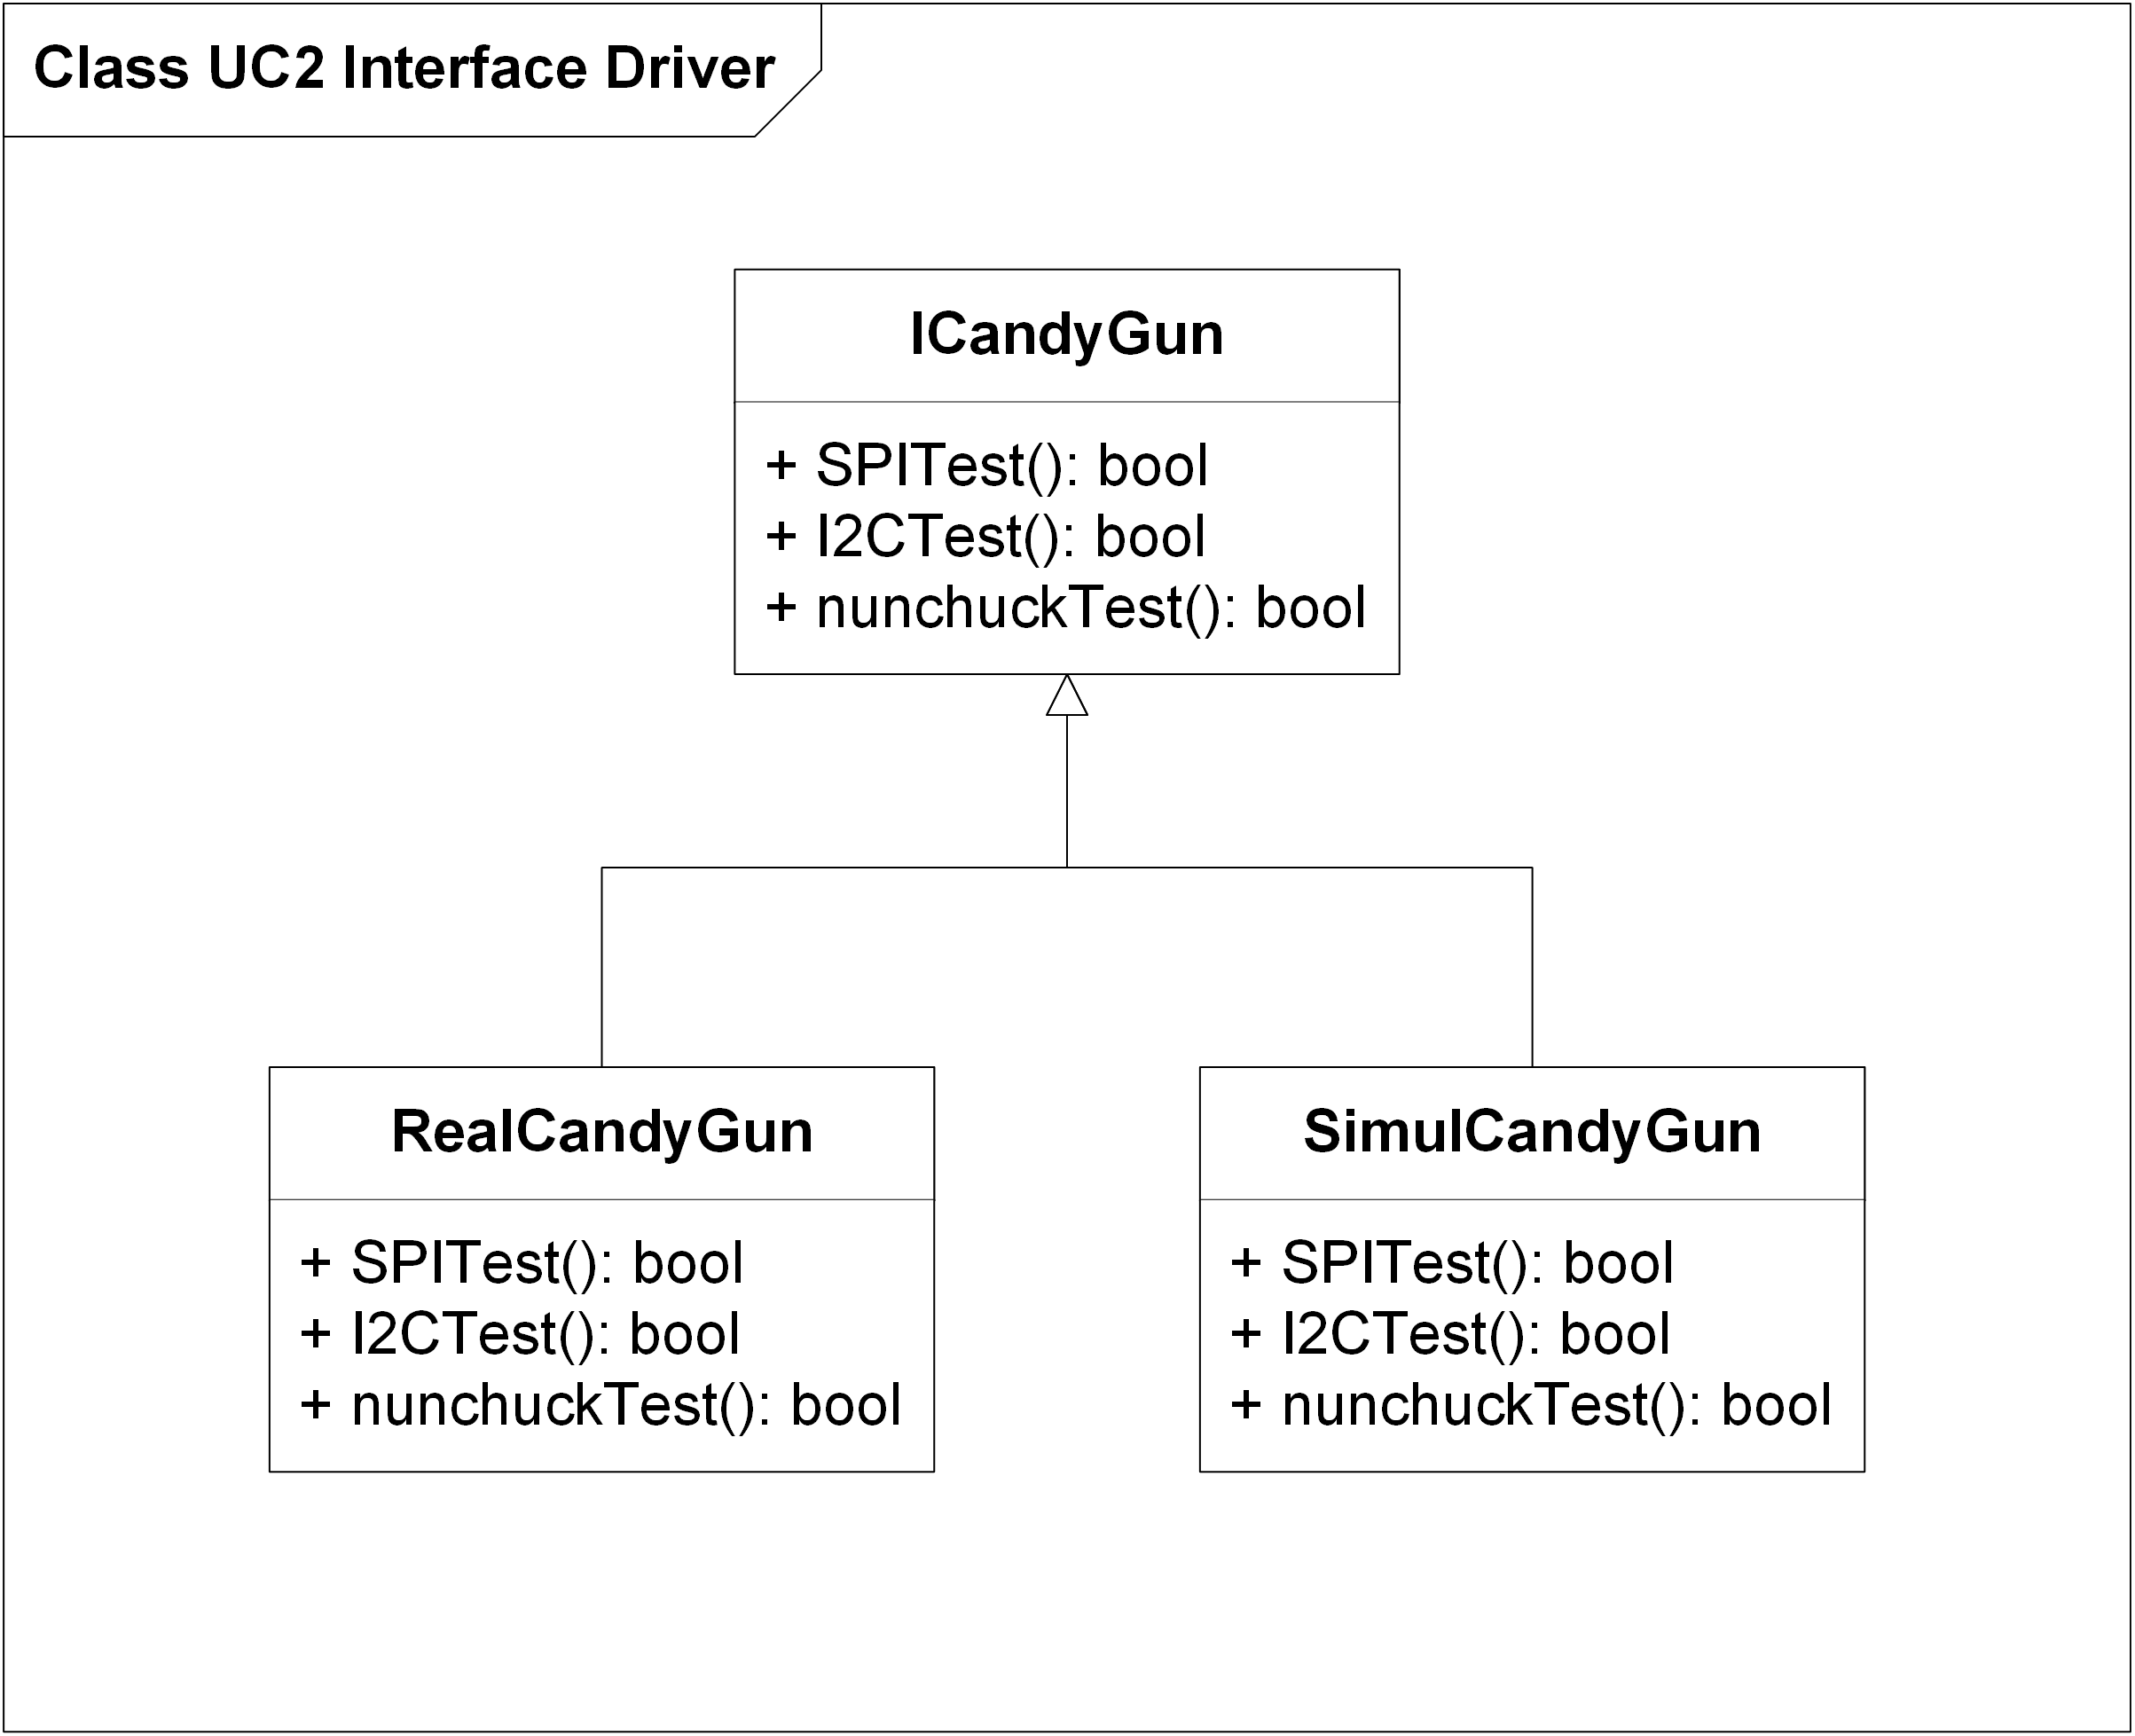
\includegraphics[width=\textwidth]{Afsnit/DesignOgImplementering/images/IdriverKlasseDiagram}
	\caption{Interface driver for UC2}
	\label{fig:idriveruc2}
\end{figure}

Basisklassen er ICandyGun. Det er en abstrakt klasse, da den udelukkende indeholder virtuelle metoder. Derudover er der to afledte klasser; SimulCandyGun og RealCandyGun. SimulCandyGun er en klasse, som implementerer metoderne til at simulere respons fra Candydriveren. Dermed kan brugergrænsefladen testes uafhængigt af de resterende dele af systemet. I RealCandyGun-klassen er metoderne implementeret efter den reelle SPI-protokol og med de nødvendige funktioner til at skrive til et kernemodul. Fx open(), close(), read () og write(). Da interface driveren er implementeret med arv, skal der ikke foretages betydelige ændringer i brugergrænsefladen, når der skiftes mellem simuleringsklassen og den rigtige version. Dermed opnås lav kobling. \\
De tre funktioner som Interface driveren indeholder i forbindelse med use case 2 (test use casen) er: SPITest(), I2CTest(), NunchuckTest(). Hver af de tre funktioner anvendes til at starte en test af de forskellige kommunikationsforbindelser: SPI, I2C og brugerinputet fra nunchucken. Alle funktionerne returnerer en bool, som enten er true eller false, alt efter om testen var succesful eller ej.\\
Brugergrænsefladen anvender interface driveren ved at inkludere headerfilerne og oprette en ICandyGun pointer, der peger på en instans af én af de to afledte klasser. Ved at pakke kommunikationen  til kernemodulet for candydriveren væk i funktioner kan brugergrænsefladen anvende funktionerne uden at kende til SPI-protokollen. Det sikrer igen lav kobling, og i tilfælde hvor det kunne ønskes, at SPI-kommunikationen kan erstattes af en anden kommunikationsform, kan det gøres uden, at der skal foretages ændringer i brugergrænsefladen.\\
 
